\documentclass{llncs}

\usepackage{url, graphicx, subfigure}
\usepackage{listings}

\begin{document}

\title{Makumba: a Framework for Rapid and Sustainable Web Development by Amateur Programmers}
\subtitle{the technological religion of a student tribe}

\author{Cristian Bogdan \inst{1} \and Rudolf Mayer\inst{2}}
%
\institute{
	School of Computer Science and Communication\\
	Royal Institute of Technology, 10044 Stockholm, Sweden\\
	\email{cristi@csc.kth.se},
\and
	Institute of Software Technology and Interactive Systems\\
	Vienna University of Technology\\
	Favoritenstrasse 9--11, Vienna, Austria\\
	\email{mayer@ifs.tuwien.ac.at}
}


\maketitle
\begin{abstract}
We present the design of a web application development framework designed together with and for non-trained programmers. The framework is proven to support sustainable, code-scalable and team-scalable development since 2002. We discuss the positive results of formal qualitative and quantitative evaluation of the framework. We then consider the aspects of the framework design that we believe are at the core of the perceived technology success. Some of these design aspects are, perhaps surprisingly, contrary to current practice in professional web development, which leads us to discuss these contradictions in more detail.
\end{abstract}

\section{Introduction}\label{sec:introduction}
Cristi: we need references/paragraphs on J2EE, Hibernate, Ruby on Rails... See the tech incantation below.

Concepts that are covered/tocuhed by Makumba and that are (hopefully) relevant for a web-engineering conference
\begin{itemize}
 \item Aspect-oriented Programming. Makumba addresses parts of AOP nicely with form validation and MDD-based authorisation.\\
  Potential reference: Kiczales, Gregor; John Lamping, Anurag Mendhekar, Chris Maeda, Cristina Lopes, Jean-Marc Loingtier, and John Irwin (1997). "Aspect-Oriented Programming". Proceedings of the European Conference on Object-Oriented Programming, vol.1241. pp. 220-�242
  \item Model-driven development. Makumba addresses this with the code generator, and more strictly with auto-forms 
  %(http://bugs.best.eu.org/cgi-bin/bugzilla/show_bug.cgi?id=781)
  \item Agile development (though agile development might seem simply as coding w/o any planning, might be contrary to the community)
  \item Rapid application development (a bit similar to agile development, but i guess older). Makumba supports this with providing the very simple DB abstration MDDs offer, with generating much of the interface from an abstract description (taglib), and maybe mainly with little overhead in configuration.
  \item Still, makumba enforces adherence to some good-practice development models, such as a simplified MVC by clearly seperating the data layer, and partly the controller.
  \item with all this, also eases software maintenance
\end{itemize}

The Intranet of an European-wide organization had just over 600 dynamic pages at its launch in 2002. The Intranet grew steadily in both size and functionality and at the end of 2008 it has almost 2000 dynamic pages. Throughout, except for a few glitches, the system was highly available and fast. Today the Intranet has around 2000 users from among the organization members, and its public part can be accessed by 4000-5000 organization customers at a time.

Such figures would not be surprising for a professional international organization, which hires or outsources professional programmers and system administrators. 
The figures are however unusual for a voluntary student organization, whose IT crew (referred to as the Tech Committee) is made of amateur voluntary student programmers who often do not study Computer Science or related subjects, or are at the early stages of their education.  
Since 2002, the Tech Committee had over 10 active members at any given time, and the Intranet was extended with more and more subsystems even if about one third of the Tech Committee membership was renewed each year. Reflection and analysis from a technology design perspective on this {\it sustainability}  is the subject matter of this paper. We assert that the design of the technology used to build the Intranet, called Makumba, is a determining factor in the Tech Committee sustainability.
Prior to Makumba introduction, the student organization had disparate IT systems, and the Tech Committee was formed in 1997 to maintain them but had much lower membership counts and was highly dependent on a few people.


Technology incantation: data driven web application development is far from being a settled matter today. on the java front: ATG dynamo, jhtml, jsp, jsf. ODMG, JDO, j2ee, back to hibernate, spring, dao, dto. We present a technology that breaks DAO and DTO and still works fine. In fact, even procedural programming seems to be needed quite seldom. The evolution of makumba isolated development around HTML and SQL. We will tell the story in this paper.

\section{Setting}\label{sec:setting}
The student organization running the Intranet of our interest was grounded in 1988 and is currently present in 79 mainly technical universities across 30 European countries. The organization grew from being present in 60 universities in 2003, and has at the moment about 2,500 members. Their aim is to organize {\it complementary education} in the form of courses and competitions for all students of the member universities (i.e. not just for its members), to assist them with {\it career support}, and to encourage the educational involvement of students by organizing symposia on engineering education aspects.
% TODO please add aims/details
The organization maintains contact with and raises funds from the European Union bodies and from a number of company partners. Internally, the organization has two statutory meetings per year and several less formal, smaller meetings in between. While most members worked on international topics only during such meetings, and for the rest they worked in their local organization chapters, since 1997 the organization was able to sustain "committees" on several topics: marketing, fund-raising, training and internal education, information technologies (the Tech Committee), and complementary education program management. The committees met in the international meetings but kept on working on their topic also in between meetings, employing e-mail and instant messaging systems, as well as dedicated tools as part of the Intranet.

The Intranet is supporting the activities of the student organization. It was assembled as an integrated system in 2002 from several systems. The {\it first} such system was an event application system for complementary education courses. The system registered student applications to the course events, and let the organization manage their acceptance (to one event out of maximum three applied for) and participation. The system had been re-built yearly since around 1993 to different levels of completeness, including several years when it failed to work and the members had to resort to manual management. The application system was based on e-mail for communication initially, and a Web-based system was devised in 1995, built using the C programming language. The system finally 'stabilized' as a Java software which was re-used for several annual editions of the complementary education program starting in 1997. This system was helping the management of the most important student organization activity and was heavily dependent on the first author until its Makumba re-implementation was completed in 2002, and still runs today.

The {\it second} system was an internal document archive and member profile management system known as the "Private Area". The system started as a set of manually maintained Web pages, storing documents produced and voted upon in international meetings, and it was automated using Lotus Notes in 1998, when internal event management was added to facilitate member application to and participation in statutory meetings and other internal events. At the time, a need for a common technology for the IT systems of the organization was recognized and Lotus Notes was intended to be that technology. However its shortcomings for the Tech Committee context were recognized and the Makumba technology was designed in response.

{\it Third} a "virtual jobfair" was built as part of the 'career support' organization mission,  allowing companies to post job adverts, and students to post their profiles. This system was among the first coordinated implementation efforts of the Tech Committee, as different from the previous spontaneous implementation endeavors by individual members. Several technologies were tried out, starting in 1997 with Lotus Notes, continuing with Java Servlet technology before the system was finally launched in 2000, using an incipient Makumba version.
% TODO, I think it was 2000, not sure how important this is, it was mostly unused for many years
% rudi: i think it was later, I'll try to dig it out

Besides heavily extending and integrating the above subsystems, several Intranet features were added since its inception: a Wiki, email archives for the organization's over 500 mailing lists, a training database, a survey-engine, a career-newletter, and a unique sign-in system that allowed students to share their accounts between the "Private Area", the course application system and the "virtual jobfair". Further, a number of team support tools were implemented, like project and task management for both international committees and local chapters, company relations management for both the fund-raising committee and the local chapters, and several specific tools for the committees, often in the form of statistical analysis of student account data, subscription to the newsletters, etc. Another major new tool is an online voting system, intended to make the statutory meetings less crowded.
%TODO more here, it feels like little was done since 2002 :)
% rudi: still not enough? :-) i can still offer: teacher access to Johnny & possibility to share materials there,;IRC chat in PA; major improvements in document archives, events management; university project (university profiles & offers on the public site); PROP aka pr-ordering pages aka a web-shop for posters & materials; an FTP storage for LBGs, integrated in PA as applet & jsp pages viewing the data, based on PA accounts; several tools for LBGs to fetch data for their local webpages;

The Tech Committee is in charge of developing and maintaining the Intranet, as well as supporting it with activities such as helpdesk. The committee also coordinates activities of interaction design for further new areas of the Intranet. Administration of the Intranet, as well as of communication systems such as e-mail are also Tech Committee responsibilities. There are two formal membership levels ("trainee" and "active member") and there is a formal coordinator, elected each year, who is also a member of the student organization overall coordination bodies. In its early (less sustainable) days, the Tech Committee consisted of 1-5 members who were mainly responsible for the individual systems and had difficulties backing each other up when they did not have time for voluntary commitment. This is similar to the present day situation of IT bodies from other student organizations in Europe and Canada who have approached the Tech Committee for know-how and technology transfer. Tech Committee membership levels increased after 2002, and new members are usually attracted in international meetings with a three-hour Makumba training, including exercises in making dynamic pages that browse Intranet data in various ways, improving existing Intranet pages, followed by assignment of more complex Intranet-related tasks.
% TODO more about the training, or after it: are they given Intranet tasks? Do they do Intranet-based exercises to change some interface or browse some Intranet data?
% rudi: in the training, they normally don't do intranet related tasks, they do completely new pages. they start from a given MDD, and then do the full range: list, object, newForm, and then for the more advanced ones also editForm, deleteLink, mak:count() & co.
% TODO rudi: not clear here, do you just want to describe the recruiting, or also the first path in ITC

\section{Methods}\label{sec:method}
We regard sustainability as a long-term matter that cannot be investigated with a short focused study. Throughout our contact with and involvement in the Tech Committee we were concerned with sustainability and at times we considered theoretical frameworks and recipes for how to achieve it, thus sustainability was an ever-present research issue for us, but also a practical issue in the community life. Both authors were active in the Tech Committee at different times (1997-2003 and 2004-2008 respectively), and {\it participant observation} was a conscious investigation approach for the first author, who also designed the Makumba technology together with Tech Committee members in a conscious act of {\it cooperative design} \cite{greenbaum_kyng91}. This paper is the occasion for a {\it reflection exercise} \cite{schon83}, on the part of the second author. Sustainability being a long-term issue, we expect other writings about it to be reflective accounts. 

We are highly aware that our first-hand involvement with the Tech Committee is a potential hinder for us producing an 'objective' account of its sustainability and on other matters of interest, and this is probably not uncommon in community-related research endeavors. We therefore complemented our personal experiences with both non-elicited and elicited data, as described below. Furthermore, our involvement having taken place {\it at different times} has resulted in a fruitful confrontation process that allowed us to depart from our personal opinions and arrive at more reliable and valid results.
%TODO more about dialog between authors
%TODO: rudi: here I'd add that we have seen a bit how it goes in other organizations, namely AEGEE, IAESTE, CFES, and to some extent bonding, though they have different settings with loads of meetings

For assessing quantitatively and qualitatively the sustainability of the Tech Committee and its practice, we regard as non-elicited data the {\it code repository} that the community has maintained, which allowed us to assess and reflect upon the progress of the Tech Committee work. The repository uses the Concurrent Versioning Systems (CVS) technology, which allows us to examine the incremental changes and additions that were made to the code, their time, and their authors. We are thus able to reconstitute the Intranet code as it was at any moment in time since 2003. A number of code analysis tools are also available for investigating CVS repositories, and we found them useful for our inquiry.

We have also elicited data from the Tech Committee members, for purposes related to the Makumba technology. In 2002 the first author evaluated the design of Makumba with a questionnaire that had 12 respondents. In 2005 the first author also ran a questionnaire with 32 respondents to asses the status of Tech Committee work and technology use, and thus indirectly look at its sustainability. Finally, both authors designed a questionnaire at the end of 2008 where 30 out of the 45 past (since 2003) and present members who were approached reflected on their activity in the Tech Committee over their whole 1-4 year-long membership period. This questionnaire provides this paper with both quantitative and qualitative data. 
% parade 2005: http://private.best.eu.org/survey/admin/listAnswers.jsp?survey=fn29yq1
% makumba 2008: http://private.best.eu.org/survey/admin/listAnswers.jsp?survey=cwu9pab

During our membership we had access to the e-mail traffic and other communication of the Tech Committee. A further form of non-elicited data is constituted by Tech Committee {\it membership lists} at different times during the committee activity since 2002. Such lists can be made by examining member profiles in the Intranet. Number of members, as well as their level of activity are useful indicators in assessing sustainability. Therefore the membership lists were complemented with levels of member activity as elicited from committee leaders and self-assessed by members themselves in questionnaires. Personal acquaintance with many of the members and knowledge of their skill evolution has come to complement this further. Some members continued on an IT career after graduation, and this was yet another indicator of their IT skills. 

To be able to better comment on our data, we will go through some conceptualizations of learning, community, practice, amateur and voluntary work, and sustainability. We will also describe in more detail the design of Makumba.

%\subsection{Amateur software development}\label{sec:amateur_devel}

% i keep this because i think that something about the parrallel with open source needs be made

%It is useful to characterize amateur software development such as hackers \cite{levy94} or open source \cite{kollock99} as amateur communities 
%because Tech Committee is a less professional (pre-professional) correspondent of such communities. 
%In such communities, code challenges are hardly exhaustible, as programming a machine leads to a rich set of contingencies, bringing along lots of 'trial and error'. 
%It is also easy to open new contingency spaces partly due to the immateriality of the working artifact, new projects, or project modules can always be started, or the existing ones can be re-organized ("refactored" in the professional jargon). For a newcomer, the complex architecture of large software projects adds to the challenge, and their skills of mastering the programming language will not be enough, they will also have to learn the way the project was organized.
%Code is shared typically via plain text messages, and carefully examined before being committed to the code repository, which suggests another amateur community feature, related to the notion of audience, the \textit{peer review} of challenge addressing. 
%Plain text is regarded as a very suitable medium for such distributed development and review efforts \cite{yamauchi00}. 
%Another important part of the community audience is its public, which can be an important motivation factor: for very generic projects it may be the world at large (e.g. in the case of an open source operating system kernel, an office suite), or very specialized professionals and amateurs in the software development field (e.g. for an open source compiler suite).

\section{Makumba, the Tech Committee tool}\label{sec:makumba}

% TODO: rudi: i think user-programmer is very misleading
Makumba was designed with influences from Lotus Notes, but without the visual programming approach that was found to be troublesome in the distributed Tech Committee setting; instead, all code is in plain text (cf. \cite{yamauchi00}). As another difference from Lotus Notes, Makumba was designed to offer as few features as possible to its user-programmers and this minimalsitic design was thought to facilitate learning. 

Makumba organizes a system in three parts. The \textit{Makumba Data Definition} (MDD) describes data structures and relations between them. MDDs are simple lists of data fields, with name and type; an example can be seen in Listing \ref{list:mdd} for the data type "Student". The \textit{JSP level} is technically a tag library for the Java Server Pages dynamic web page technology, which allows displaying and changing the data stored in a database and described in MDDs. Finally the \textit{business logic} (BL) describes, in the Java programming language, % (mostly its procedural features)
"business rules" that restrict the changing of data, and provide authentication and authorization mechanisms. The JSP level, illustrated in Listing 2, provides for a combination of HTML and a subset of SQL (Structured Query Language). The example shows a list of students and, for each student, their completed studies. The data for this list is described in the aforementioned "Student" MDD. Notably the SQL data combinations (so-called joins) and data selections (so-called projections) are generated automatically from notations like "s.education" and "s.surname" respectively. Therefore working with a Makumba JSP would typically not require as much knowledge as using SQL by itself.

\lstset{basicstyle=\small, captionpos=b, caption=Makumba Data Definition "Student", label=list:mdd, frame=shadowbox}
\begin{lstlisting}
name = char[50]
birthdate = date
hobbies = text

education = set
education->name = char[50]
education->university = ptr University
\end{lstlisting}

\lstset{basicstyle=\small, captionpos=b, caption=Example of viewing data with the Makumba JSP tag library, label=list:mak, frame=shadowbox}
\begin{lstlisting}
<mak:list from="Student s">
  Name: <mak:value expr="s.name"/> <br/>
  Born on: <mak:value expr="s.birthdate"/><br/>
  Completed studies:
  <mak:list from="s.education e"
  	    where="e.graduationDate < now()">
    <mak:value expr="e.name"/>
    (<mak:value expr="e.university.name"/>),
  </mak:list>
  <br/>
</mak:list>
\end{lstlisting}


Through this design, the assumption was that it will be easy for students to read MDDs, and based on that, it will be possible for them to combine HTML and a subset of SQL (itself based on natural language) which they might know prior to start working with Makumba or might learn "on the job". Later on, they would become interested in writing new business rules, and might learn procedural Java for that, maybe using previous knowledge of another procedural programming language. This then would be the "learning path" assumed for a Makumba practitioner.

Initially Makumba was designed and developer under another, more neutral name ("Metadata"). When a more specific name was sought, designers remembered of a name that was well-known to many student organization members: the Makumba party. The name was known but not the actual meaning because members who had attended a Makumba party usually described as like below, without further detail. 
\begin{quotation}
	"You enter a room, the lights are turned off and then somebody tells the Makumba joke."
\end{quotation}

Ironically, the main Makumba designer had never attended a Makumba party, but knowing about its existence and its fame within the organization was enough to decide on the name.

\section{Sustainability of the Tech Committee}\label{sec:techCommittee}
\begin{table}
	\centering
	% TODO: explain LOC, etc? explain that all data is measured at the beginning of the year?
	% TODO: explain the drop from 2008 to 2009 needed? (due to removal of old BCC & public website pages in 2008, new ones have been added since late 2007, thus there were some ``duplicates'')
	\begin{tabular}{c|r|r|r|r|r|r}
		\hline
		\hline
		Year	& MDD	& JSP	& BL	& \# files	& LOC		& CVS	 \\
		\hline
		\hline
		2002 	& 42	& 676	& 80	& 801		& 78479 	& N/A	 \\ 
		\hline
		2003 	& 52	& 961	& 116	& 1132		& 104805 	& 1143	 \\ 
		\hline
		2004 	& 64	& 1208	& 140	& 1415		& 127873 	& 702	 \\ 
		\hline
		2005 	& 76	& 1354	& 190	& 1628		& 151801 	& 1324	 \\ 
		\hline
		2006 	& 99	& 1719	& 229	& 2062		& 175315 	& 1632	 \\ 
		\hline
		2007 	& 111	& 2135	& 287	& 2559		& 219456 	& 2391	 \\ 
		\hline
		2008 	& 114	& 1860	& 289	& 2304		& 196867 	& 1898	 \\ 
		\hline
		
% old data, # files & LOC from CVS-stat
% 		Year		& \# files 		& LOC		& MDDs	& JSPs	& BL \\
% 		\hline
% 		\hline
% 		2003		& 850			& 55,000	& 42	& 729	& 80\\
% 		\hline
% 		2004		& 1,200			& 75,000	& 52	& 1097	& 116\\
% 		\hline
% 		2005		& 1,700			& 85,000	& 64	& 1388	& 140\\
% 		\hline
% 		2006		& 2,300			& 132,000	& 76	& 1564	& 190\\
% 		\hline
% 		2007		& 3,050			& 200,000	& 99	& 2057	& 229\\
% 		\hline
% 		2008		& 3,550			& 305,000	& 111	& 2526	& 287\\
% 		\hline
% 		2009		& 3,750			& 312,000	& 114	& 2303	& 289\\
		\hline
		\hline
	\end{tabular}
	\caption{Size of the Intranet}
	\label{tab:intranet-size}
\end{table} 

Let us first illustrate the Tech Committee activity in what we perceive as its sustainable period. Table~\ref{tab:intranet-size} shows the evolution of the size of The Intranet since its launch seven years ago, detailed for the different technological levels MDD, JSP and BL. Additionally, the total number of code files is shown, along with the total lines of code (LOC).  Figure 1 shows the evolution of the code figures graphically. It is worth noting that there was a rather high amount of data definition (MDD) files defined in the beginning of The Intranet, representing data used in the first three sub-systems. Even though more data definitions have been added over time, a certain saturation level has been reached in the last years, with only minor additions. It is not unexpected that the data definitions of an organization (its "domain model") change seldom after an initial development time. 
As different from that, the amount of Business Logic (BL) files has continuously increased, with a leveling in the last year.
% TODO: rudi: i really think this explanation of the decrease is wrong; we didn't get rid of any file due to refactoring, we surely got rid of some LOC, though. in any case, we should explain this by the true reasons, i.e. having for some time a new application redesigned, and both versions in the repository.
This leveling, as well as a JSP file number decrease, are due to the Tech Committee finding the time to re-organize (refactor) their code without adding functionality, but simplifying it in the process, thereby allowing future members to understand it easier, and making it possible to implement more powerful features over the new, improved, code structure. Finding the time and resources for refactoring is itself a sign of sustainability.

% TODO: rudi: show which axis is for which data
\begin{figure}\label{fig:intranet-size}
   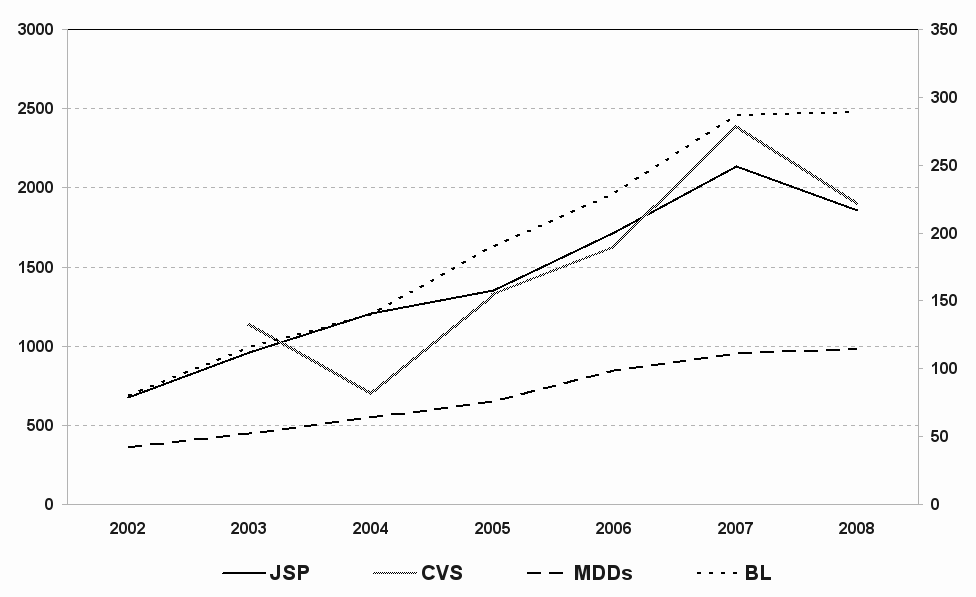
\includegraphics[width=0.98\columnwidth]{figures/SizeChart}
  \caption{Size of the Intranet}
\end{figure} 

% TODO: describe why ``active'' column might have smaller numbers than others..
Table~\ref{tab:itd-members} illustrates the number of active members in the Tech Committee since 2003, differentiated on the different levels of Makumba, and on their activity in newcomer (``peripheral'') and old-timer (``core'') members. This data was  extracted on the one hand from the latest questionnaire filled in by the members, and then refined and amended by some of the committee coordinators (for the year 2003, only the total number of active core and peripheral members could be estimated). It is interesting to note that while the overall number of active members increased over the years and stabilized in the last years, the (relative) number of members working on data definitions (MDD) was rather decreasing; this might be explained with the arrival at data maturity level as described above, and thus less work and challenges to take for the Tech Committee members, while plenty of challenge is left at other levels. An important sign of sustainability as we characterized it earlier is the sufficient number of members at both novice (peripheral) and expert (core) members active at all the Makumba usage levels at all times. The "learning paths" are thus well populated with community members.

\begin{table}
	\centering
	\begin{tabular}{c|r|r|r|r|r|r|r|r|}
		\hline
		\hline
		Year 		& \multicolumn{2}{c|}{MDD} & \multicolumn{2}{c|}{JSP}	& \multicolumn{2}{c|}{BL}	& \multicolumn{2}{c|}{Active}	\\
					& Per & Core				& Per & Core				& Per & Core				& Per & Core	\\
		\hline
		\hline
		2003 &   &   &   &   &   &   & 4 & 5 \\
		\hline
		2004 & 3 & 4 & 7 & 3 & 3 & 3 & 6 & 5 \\
		\hline
		2005 & 5 & 6 & 8 & 11 & 7 & 3 & 8 & 13 \\
		\hline
		2006 & 7 & 8 & 9 & 12 & 9 & 3 & 10 & 12 \\
		\hline
		2007 & 7 & 7 & 14 & 9 & 10 & 5 & 12 & 11 \\
		\hline
		2008 & 6 & 5 & 13 & 7 & 6 & 7 & 12 & 8 \\
		\hline
		\hline
% Summer meetings
% 2003: http://private.best.eu.org/events/event.jsp?event=21-C-CJ-COM
% 2004: http://private.best.eu.org/events/event.jsp?event=22-C-RI-COM
% 2005: http://private.best.eu.org/events/event.jsp?event=23-C-LD-COM
% 2006: http://private.best.eu.org/events/event.jsp?event=24-C-SF-COM
% 2007: http://private.best.eu.org/events/event.jsp?event=25-C-TM-COM
% 2008: http://private.best.eu.org/events/event.jsp?event=26-C-BE-COM
	\end{tabular}
	\caption{Members in the Tech Committee}
	\label{tab:itd-members}
\end{table} 

\subsection{Survey}\label{sec:techCommittee-survey}
A survey was conducted among current and former members of the Tech Committee in the end of 2008, and filled in by 30 members. The time of Tech Committee membership ranges from their activity starting around 2001, to fresh members that just joined in the second half of 2008. Also the educational background is diverse -- 13 members study computer science, computer engineering or informatics; the other respondents follow various other curricula, ranging from mechanical engineering to physics and biomedical engineering. Also, the membership duration in the committee varies, from 6 members that were active for around four years, to members that were (or currently are) active for one to two years. Most members had no knowledge of Makumba before joining.

The questionaire consisted of 53 questions. The main focus was on gathering an understanding of the learning aspect of Makumba in the context of the Tech Committee, thus the participants were asked to answer several questions on their self-assessed skill level on database design, SQL, general programming, Java, and three aspects of Makumba: JSP pages to view data, JSP pages to change (create, edit, and delete) data, and business logics (BL). The questions were asked repeatedly for several different points in time, namely when joining the committee, and after the first, second, third and fourth year of membership, and allowed answers from ``no skills'' via ``little knowledge'', ``some experience'' and ``experienced'' to ``master''. To balance the self-assessments and to facilitate recall, the participants were further asked to estimate their contribution to the committee in that year, and to list the projects and technologies that they worked with in that year. Also to improve the quality of the self assessment, members were informed that the committee coordinators from their time of activity will review their answers.

Figure 2 shows the averaged skill levels of all the members at different points in time, separated for three Makumba usage aspects: JSP for viewing data, JSP for modifying data, and BL. It can be observed that apparently, learning to view and display data in JSP level is faster than handling forms to create, edit, and delete data, while Business Logics are the most difficult concept, especially in the first two years of membership. Most members that stay in the committee for a longer period, however, master all levels of Makumba almost equally well, but that is not a case of challenge exhaustion as they can (and many do) continue working on the internals of Makumba itself  as a next step. While MDD editing skills are less and less actual, we can consider that currently the learning path milestones in the Tech Committee are: JSP viewing data, JSP changing data and BL. To further illustrate the member skill evolutions, we have selected the charts of four individual members in Figure 3. This also shows that, although the dynamics vary a lot, the JSP data-changing skills almost always lag behind the JSP data view skills, and BL skill is acquired last. 

Overall, the per-year self-assessment results suggest that the learning path designed into Makumba has achieved its goal, allowing for members to have an easy start by visualizing data in JSP (which also requires MDD understanding), then starting to change data and finally learning how to write business rules in Java.

\begin{figure}
   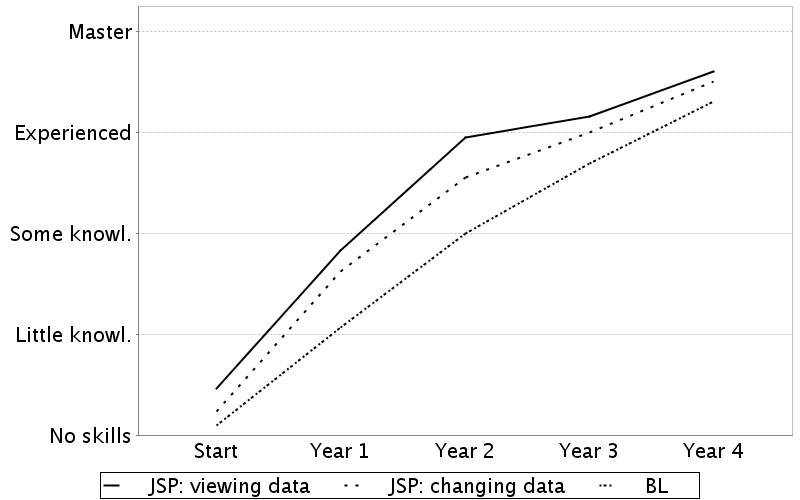
\includegraphics[width=0.98\columnwidth]{figures/learning-technologies}
  \caption{Learning curve for different aspects of Makumba}
  \label{fig:learning-technologies}
\end{figure} 

% \begin{figure}\label{fig:learning-members}
%   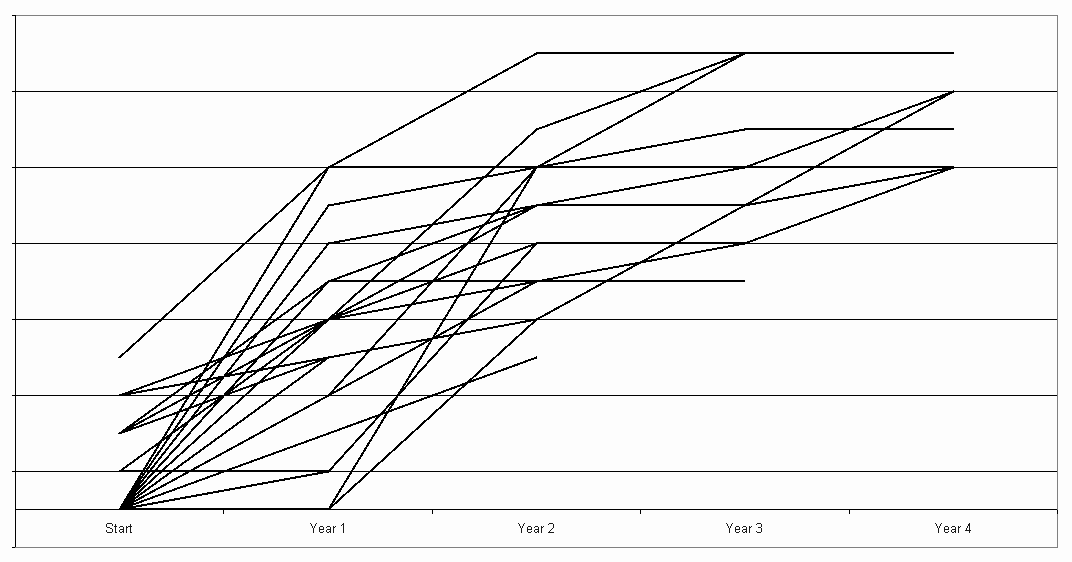
\includegraphics[width=0.98\columnwidth]{figures/learning-members}
%   \caption{Skill development of the survey respondents over the years}
% \end{figure} 

\begin{figure}
  \label{fig:learning-members}
  \caption{Skill development of selected survey respondents}
  \subfigure[Julian]{
     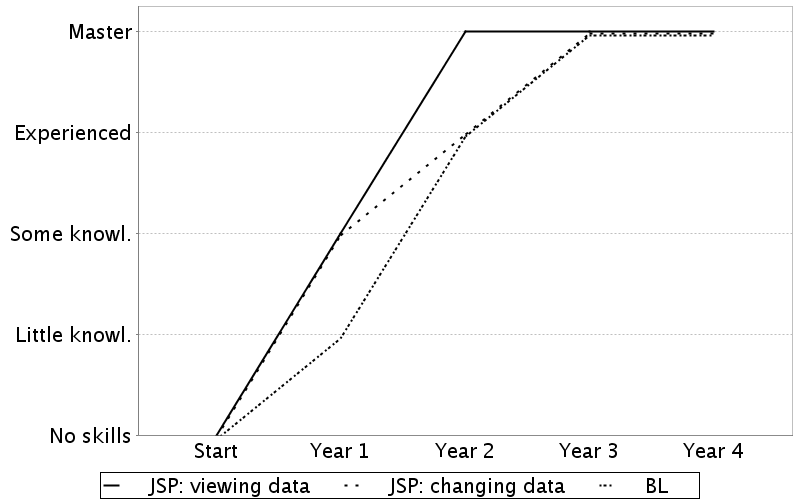
\includegraphics[width=0.47\textwidth]{figures/Joao}
    \label{fig:learning-members-joao}
  }
  \subfigure[Peter]{
     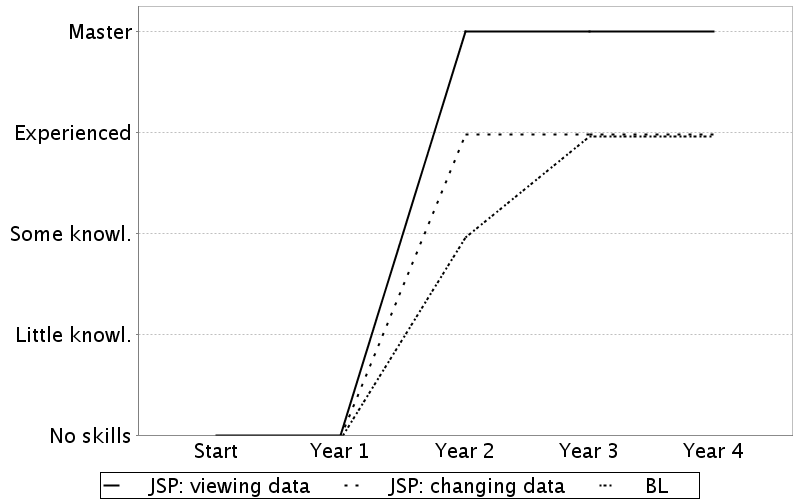
\includegraphics[width=0.47\textwidth]{figures/Priit}
    \label{fig:learning-members-priit}
  }
  \\
  \subfigure[Kim]{
     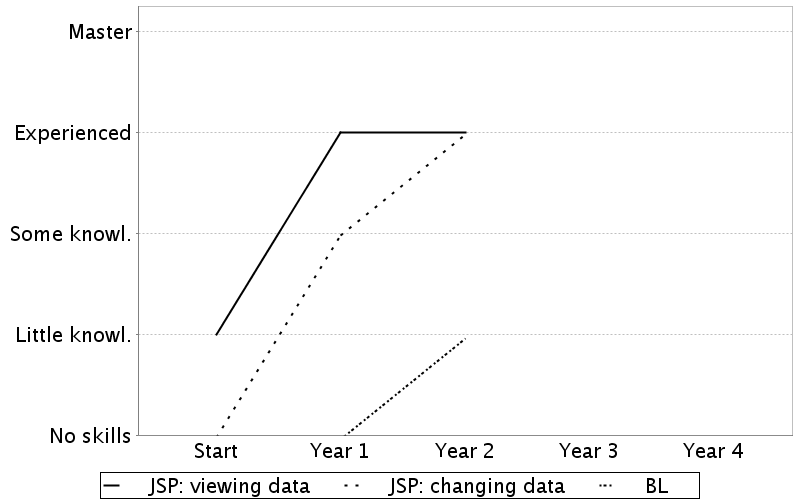
\includegraphics[width=0.47\textwidth]{figures/Karina}
    \label{fig:learning-members-karina}
  }
  \subfigure[Sam]{
     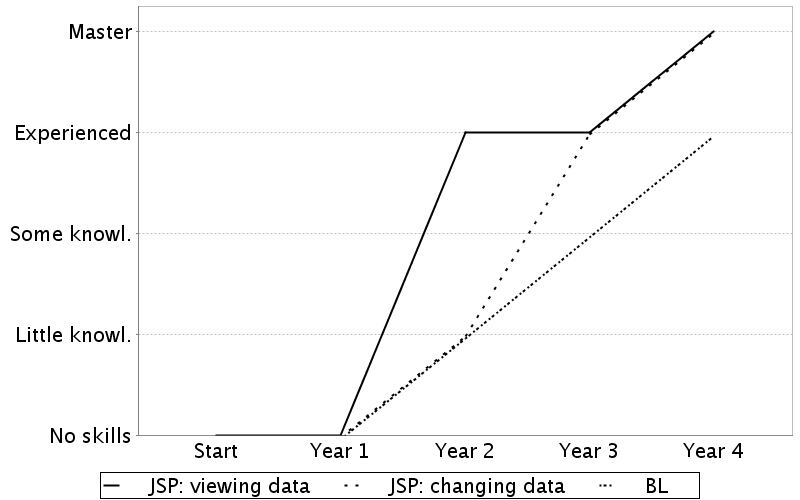
\includegraphics[width=0.47\textwidth]{figures/Stefan}
    \label{fig:learning-members-stefan}
  }
\end{figure} 




Two open questions concluded the questionnaire. We will comment them briefly here, and elaborate in the discussion. The first one aimed at helping to assess how the members experience learning technologies in the Tech Committee. Several respondents emphasized the \textit{simplicity} and conciseness of Makumba code, therefore easiness to start working with, in various ways: as an intuitive link between code and result,  or as a praise to simplicity perceived as being able to express things in only one way, with a direct reference to people coming into and leaving the Tech Committee,  or as a technology that provides for rapid achievement, thereby encouraging further involvement. It is important for the Tech Committee in the international meetings to 'catch' people fast, by allowing them to realize that they can do something, that they can contribute. If this would not happen fast, the prospective new member might lose interest and maybe try to join another international team where contribution is more facile. A respondent emphasizes that "there is life" beyond the first simple steps, i.e. there are more complex things to be done, and Makumba accommodates for these as well. Several respondents compare Makumba with other Web development frameworks in this regard. More than one respondent referred explicitly to "non-IT people", thereby emphasizing the suitability for amateur settings.

% http://private.best.eu.org/survey/viewStatistics.jsp?survey=cwu9pab&graphs=true&comments=true
%\begin{quotation}
% 	"I would say that the code is very close to the result ('what you code is what you get'), or at least, very logically connected."

%	"One big advantage is the syntax, which makes it straight forward to understand other people's work. With Makumba, it doesn't happen so often that 2 people write totally different pieces of code for the same feature, and this is very useful for [the student organization] (where people change very often)."

%	 "anybody is able to get a working page after 10 minutes of theory and 5 minutes of practice. That's provide motivation to do more difficult features."

%	"[...] allowing to reach very quickly decent results with its basic features (allowing new joiners not to get tired of the learning effort and to contribute quickly) while also providing more powerful stuff for advanced users (allowing them to still find new challenges)."
%	
%	"All the other frameworks and technologies I know (Struts, PHP + templating engine, Zope) require a higher degree of computer technologies knowledge to achieve similar results. This might be changing with new frameworks like Ruby on Rails in which the model definition is done in a similar way as in Makumba, but still I think Ruby on Rails' learning curve is steeper than Makumba's"
%		
%	"Makumba being specifically designed for web applications, it is both extremely simple to learn for the basics - easier than PHP, especially for non-programmers - mainly through the easy interactions with databases; yet can be as powerful as any other language"
%	
%	"But the main advantage is that everyone \textit{can} learn, without too much of a technological background. I think that for [Tech Committee], or for any organization who wants to involve non-IT people in the development of their applications, the use of Makumba can make things much easier."

%\end{quotation}


Respondents refer to their learning primarily from other members, sometimes even without explicit training and without even mastering the basics of the entry-level skill (HTML and SQL). Also learning by reading a mailing list is mentioned. Other informants report having asked questions on the Tech Committee mailing list and getting a multitude of good answers, also usable in the professional life of the then-amateur.


%\begin{quotation}
%% 	% rudi: community learning, but too focused on events. ? good that it's mentioned that HTML & SQL are not needed
%	"I didn't attend any organised Makumba training, but learned the basics during events, in the first year. It was quite easy, although I didn't even know HTML or SQL when joining [the Tech Committee]. On the first 1-2 projects, I was directly helped by [the Tech Committee]'s experienced members. Afterwards, I started following also the emails and learned a lot from other people's problems/experiences."
%	
%	"The [Tech Committee] community is helpful, it is very easy to learn new technologies. I think makumba gives a very good starting point for learning web programming (separation of concerns, data model design). Everything that I learned in [Tech Committee] has proved to be true also in the professional web development world. "
%\end{quotation}


% \begin{quotation}
%	% rudi: mentions only ITD
% 	I usually learn by reading code and trying to reform it in a way that suits what i want to do. ITD is good at this part, since all our code is available and it's easy to find a place that something similar was done before. 
% \end{quotation}

Learning by reading examples (existing code) is emphasized by most respondents. Knowing how the Intranet is organized helps to find relevant code:
%\begin{quotation}
%	"Learning is easy thanks to a lot of examples: for most of the tasks I could find another place where a similar feature had been implemented. Having a good knowledge about [the student organization] IT systems helps more than having strong programming skills. Other [Tech Committee] members also very often help and give advice when a problem or mistake occurs. "
%\end{quotation}

A problem with learning Makumba is raised: since it is little known outside the student organization, there is no chance that some joining members already come in the Tech Comittee with the skill:
%\begin{quotation}
%%, altough that involves dealing with Java, which is immediately more complicated - but not more complicated than any complex operation with any language.
%	"The main disadvantage is that everyone must learn it, since it is quite different from other web technologies."
%		% (provided that we keep having nerd masters to maintain and update it :p) 
%\end{quotation}


The last question asked the respondents for a comparison of Makumba with other technologies and frameworks aimed for web development. Many of the former or present members of the Tech Committee, currently working in IT jobs, were able to provide comparisons from a qualified professional perspective, with references to related technologies. Notably a number of members make architectural remarks, referring to some technical imperfections of Makumba, which does not provide a good separation between data ("model"), its visualizations ("view") and the data change mechanisms ("controller"), within a widely accepted professional paradigm, called Model-View-Controller. However most respondents regard this as an asset in the end, leading to easier programmer access to the data and higher maintainability.

%\begin{quotation}
%	"Mak is significantly more suitable for [the Tech Committee] than anything else I've seen, despite the horrible inflexibility of the J2EE platform. Most other frameworks/setups insist on a very clear separation between the model and the view, and in most situations, this makes sense. However, by moving certain typically controller-world operations, such as database queries, to the view \textbf{in a simple and accessible way}, pages become much more maintainable without very strong documentation discipline, because they somewhat self-document."

%	"atm. I can't think of frameworks that do mix view and model, i.e. view and data query. they all go through a DAO layer, which would break the "what you code is what you get". other frameworks also do have a lot of configuration overhead and rely on Java, which make it difficult for beginners to grasp. e.g. Struts needs to have several files changed in order to get a form to work, which is not so straightforward and slows down the "try and error" process." 
%	
%	"Technology-wise, I love Makumba as how it's designed -- the whole way the view/controller separation is less sharp than in other frameworks, how this is made very accessible and maintainable using the Makumba tag library, and how in the end this makes a large intranet maintainable by a community of people of variable skills. "

%\end{quotation}

\section{Discussion}\label{sec:disco}
We should first mention that we cannot deny the merits of the non-technological aspects of the Tech Committee work and organization that contributed to its sustainability: the managerial skills of its leaders and experienced members, or the well-organized mentoring of the newcomers, are all aspects that surely help sustaining the Tech Committee practice. However, our data (including explicit statements from members of different generations) shows that Makumba's learning-oriented design and the meanings associated with Makumba in the student community play a crucial role in the Tech Committee sustainability.

Our data shows that designing a programming technology that allows member activity at various levels of skill, thereby prescribing a learning path for the members of the amateur community of practice, allows for sustainability of the amateur programming practice. In the case in point, we saw that the 'learning departments' of the setting, corresponding to the different programming languages used, were well populated at all times, in all our annual counts,  even if members left the setting every year while others joined. We can recommend as a design implication to design 'skill-modular' technologies, with 'modules' that require different levels of skill, with the first such module having a low learning threshold (HTML and simplified SQL-queries in the Makumba case), in order to provide for challenge addressability, and the next modules providing new challenge levels (e.g. BL in the Makumba case, with the procedural Java skill to be learned), thereby helping towards challenge inexhaustibility \cite{bogdan_bowers07}. Such learning modules with new challenges also provide for progressing from the periphery to the core, thus molding themselves well on Community of Practice social learning. The technology can then, as we believe Makumba does, be part of the \textit{configuration} process emphasized by Lave and Wenger \cite{lave_wenger91}. Especially for the entry-level skill modules (the JSP level of Makumba), \textit{code legibility} is an important design feature for an amateur programming technology, in such a context of learning in doing, from peers, or from the artifacts they produced. 
% TODO: rudi: isn't `` is not unexpected'' a bit too weak as a statement?
Most of our respondents mention looking at a working example when performing a task, and this is not unexpected in a Community of Practice. A major part of the Makumba JSP level simplicity and legibility is inherited from the corresponding feature of SQL queries, as legibility and intuitiveness were among its design principles, since it is based on natural language. Members who do not know SQL simply have to rely on their English to find their way around initially. This is further helped by Makumba JSP using a simplified form of SQL queries. Using plain text code rather than visual programming further helps the sharing and understanding of existing examples \cite{yamauchi00}. We will also emphasize here the importance of an \textit{amateur programming experimentation} (cf.  \cite{bogdan_bowers07} for experimentation with amateur radio equipment).
% TODO: rudi: actually, no one really works in production...
Few programmers work on the actual 'officially running' system, instead they work on a copy of it running with some example data. The lower the skill available, the more important the space for experimentation becomes, as a space for making initial mistakes, trial and error, and low-risk attempts to find solutions. It is difficult to imagine what Makumba programming would have been without the Tech Committee members' sandbox.

We were however not satisfied when discussing our data that this theoretical 'skill modularity' picture captures the Tech Committee sustainability entirely.The first author, who proposed it, has never actually been active in the sustainable period of the Tech Committee, and has coded little of the the Makumba Intranet. It was the second author, along with former and present Tech Committee leaders during its sustainable days, who pointed out  several other aspects that lead to sustainability, some of which were confirmed by questionnaire respondents. First, the student organization regards Makumba as being something that \textit{belongs} to them. It is something that they give to the world therefore it is a way for them to relate to a \textit{public} \cite{stebbins79}, or a wide \textit{audience} \cite{bogdan03}, thereby increasing amateur motivation. Entering the Tech Committee gives one a privilege to work with a technology that is unique, and designed by previous Tech Committee generations. Entering the Tech Comittee also means being part of the team who had in 1995 an automated online application system at a time when many companies barely had a static website. While such an early achievement is not directly related to Makumba, it emphasizes the Tech Committee long-lasting tradition in the area of dynamic Web applications, Makumba's application domain, and is supplemented by other similar \textit{war stories} \cite{orr96} that have a role in learning, but also in creating a sense of belonging. Furthermore, entering the Tech Committee often means attending a Makumba party, one of these mysterious events that other people talked about but never wanted to give details. This reminds us of an \textit{initiation rite} \cite{vanGennep60} and plays a role in attracting new blood to the committee.
%TODO: rudi: shouldn't this rather be ``an inspiring act''? how can it be inspired in retrospect?
In retrospect, choosing the Makumba name in favor of other, more technology-oriented but less student-community-oriented names was an inspired act. This teaches us that, while skill modularity has its merits, it can always use complementation from cultural meanings ascribed to the technology within the community: traditions, war stories, rituals, world-unique specificities. An implication then is to try to link the technology with community meaning. If this was possible to achieve (albeit somewhat accidentally) for such an intricate thing as a web development framework by a simple act of baptizing, it could work for many other technologies.

The relative uniqueness of Makumba to the student organization has an interesting consequence: since it is not a well-known technology, there are very few Tech Committee members who already know the technology when they join the committee, so they have to learn it when they join, at the same time as they come in contact with the traditions and rites associated with it. As there are not many resources dedicated to Makumba on the Internet, they have to resort to their fellow Tech Committee members, thus being 'forced into socialization', and thus fueling peer learning.
%TODO rudi: maybe another advantage is that they cannot bring in bad programming habbits/styles.. ?


Reflection on Makumba as a technology for \textit{pre-professionals} \cite{stebbins79} leads us to two apparently contradictory considerations. On the one hand, Makumba imposes a professional rule, preventing the amateurs from mixing business rules with data views.  The two are programmed in very different languages, requiring different skills, and different skills levels, making  it difficult for the amateurs to even attempt to mix them. Many technologies in use by amateurs (like PHP) do not enforce this separation, leading to lack of \textit{code scaleability} of application development: applications can be started fast, like with Makumba, but once they grow large, problems start to occur due to not enforcing this major principle, affecting in the end sustainability. On the other hand, another professional rule, the separation of data view from data access is violated by Makumba, as emphasized by several former members, currently professionals. Ironically, the two rules are part of the same professional design pattern, the Model-View-Controller. \textit{Selecting relevant professional principles} is thus yet another design implication that we draw for amateur technology, and as the example shows, it can lead to fine-grained decisions. In other words, even if the professional counterpart is a potential role-model to be followed by the amateurs \cite{stebbins79}, not all its aspects will be useful in the amateur programming setting. We can draw a simple consequence of this implication: many professional technology designer use "more is better" as a principle in designing a feature set. In an amateur community, like it happened for the Tech Committee with Lotus Notes, members trying to employ such a technology would have a hard time choosing the feature they need. The small number of Makumba data types as well as the small amount of keywords in languages used (HTML, SQL-query) come to suggest that "more is better" is not a good professional principle to select, as it doesn't fit the amateur learning situation, where members need to get involved (and get some sense of achievement) fast. 

A further feature that we can recommend for amateur programming technologies, related to code legibility, is to provide for \textit{easy code navigation}.  As emphasized by some respondents, Makumba has fewer types of files than professional technologies in the same application domain, therefore requiring less navigation between files when performing a task. Although this sometimes breaks the professional principle of separation of concerns (like data access concern and data view concern, as illustrated above) it helps the novices to make easier progress, and achieve better orientation when contributing to a large project like the Intranet. Furthermore, this source file compactness, especially at the JSP level, leads to little interdependency between the JSP source files (i.e. changing one such file is not prone to affect the working of many others), which helps when several of amateur programmers work on different parts of the Intranet, as they are not prone to affect each other's work, and thus the likely mistakes that a novice makes will not affect his or her peers. Such \textit{team scaleability} is ideal for amateur programming sustainability.

\section{Conclusions}\label{sec:conclusions}
We have described the sustainability of an amateur programming group, and examined it as an Amateur Community and as a Community of Practice. Based on this framework and on data collected over several years, we proposed several technology design implications for achieving sustainable practice in communities. We suggest that technologies should be learning-oriented, more precisely they should be organized around skill modules. We further suggest that technologies should be associated with community traditions, rituals and specificities. Finally, we suggest that a careful selection must be done from among the principles used within professional counterpart of the amateur community. Such a selection should also be made with learning in mind: professional principles can be broken at the expense of easier learning, yet other professional principles must be enforced to ensure long-term sustainability.

%ACKNOWLEDGMENTS are optional
\section{Acknowledgments}\label{sec:acknowledgments}
Thanks to the students, members and associates of the Tech Committee who have worked hard to overcome Makumba imperfections and to make the Intranet what it is today, while also taking time to answer our surveys.  Thanks are also due to all the Makumba contributors.  Anonymous1 and Anonymous2 have supervised this work with good advice during the crucial Makumba design phases.


\bibliographystyle{plain}
\bibliography{icwe2009-makumba} 

\end{document}
